\documentclass[12pt, titlepage]{article}

\usepackage{fullpage}
\usepackage[round]{natbib}
\usepackage{multirow}
\usepackage{booktabs}
\usepackage{tabularx}
\usepackage{graphicx}
\usepackage{float}
\usepackage{hyperref}
\hypersetup{
    colorlinks,
    citecolor=blue,
    filecolor=black,
    linkcolor=red,
    urlcolor=blue
}

%% Comments

\usepackage{color}

\newif\ifcomments\commentstrue %displays comments
%\newif\ifcomments\commentsfalse %so that comments do not display

\ifcomments
\newcommand{\authornote}[3]{\textcolor{#1}{[#3 ---#2]}}
\newcommand{\todo}[1]{\textcolor{red}{[TODO: #1]}}
\else
\newcommand{\authornote}[3]{}
\newcommand{\todo}[1]{}
\fi

\newcommand{\wss}[1]{\authornote{blue}{SS}{#1}} 
\newcommand{\plt}[1]{\authornote{magenta}{TPLT}{#1}} %For explanation of the template
\newcommand{\an}[1]{\authornote{cyan}{Author}{#1}}

%% Common Parts

\newcommand{\progname}{PCD: Partially Covered Detection of Obscured People using Point Cloud Data} % PUT YOUR PROGRAM NAME HERE
\newcommand{\authname}{Team \#14, PCD
\\ Tarnveer Takhtar
\\ Matthew Bradbury
\\ Harman Bassi
\\ Kyen So} % AUTHOR NAMES                  

\usepackage{hyperref}
    \hypersetup{colorlinks=true, linkcolor=blue, citecolor=blue, filecolor=blue,
                urlcolor=blue, unicode=false}
    \urlstyle{same}

\usepackage{indentfirst}                              


\newcounter{acnum}
\newcommand{\actheacnum}{AC\theacnum}
\newcommand{\acref}[1]{AC\ref{#1}}

\newcounter{ucnum}
\newcommand{\uctheucnum}{UC\theucnum}
\newcommand{\uref}[1]{UC\ref{#1}}

\newcounter{mnum}
\newcommand{\mthemnum}{M\themnum}
\newcommand{\mref}[1]{M\ref{#1}}

\begin{document}

\title{Module Guide for \progname{}} 
\author{\authname}
\date{\today}

\maketitle

\pagenumbering{roman}

\section{Revision History}

\begin{tabularx}{\textwidth}{p{3cm}p{2cm}X}
\toprule {\bf Date} & {\bf Version} & {\bf Notes}\\
\midrule
Jan 17, 2025 & 1.0 & Initial Draft\\
\bottomrule
\end{tabularx}

\newpage

\section{Reference Material}

This section records information for easy reference.

\subsection{Abbreviations and Acronyms}

\renewcommand{\arraystretch}{1.2}
\begin{tabular}{l l} 
  \toprule		
  \textbf{symbol} & \textbf{description}\\
  \midrule 
  AC & Anticipated Change\\
  DAG & Directed Acyclic Graph \\
  M & Module \\
  MG & Module Guide \\
  OS & Operating System \\
  R & Requirement\\
  SC & Scientific Computing \\
  SRS & Software Requirements Specification\\
  PCD & Partially Covered Detection Program \\
  PCL & Point Cloud Library \\
  CLI & Command Line Interface \\
  GUI & Graphical User Interface \\
  UC & Unlikely Change \\

  \bottomrule
\end{tabular}\\

\newpage

\tableofcontents

\listoftables

\listoffigures

\newpage

\pagenumbering{arabic}

\section{Introduction}

Decomposing a system into modules is a commonly accepted approach to developing
software.  A module is a work assignment for a programmer or programming
team~\citep{ParnasEtAl1984}.  We advocate a decomposition
based on the principle of information hiding~\citep{Parnas1972a}.  This
principle supports design for change, because the ``secrets'' that each module
hides represent likely future changes.  Design for change is valuable in SC,
where modifications are frequent, especially during initial development as the
solution space is explored.  

Our design follows the rules layed out by \citet{ParnasEtAl1984}, as follows:
\begin{itemize}
\item System details that are likely to change independently should be the
  secrets of separate modules.
\item Each data structure is implemented in only one module.
\item Any other program that requires information stored in a module's data
  structures must obtain it by calling access programs belonging to that module.
\end{itemize}

After completing the first stage of the design, the Software Requirements
Specification (SRS), the Module Guide (MG) is developed~\citep{ParnasEtAl1984}. The MG
specifies the modular structure of the system and is intended to allow both
designers and maintainers to easily identify the parts of the software.  The
potential readers of this document are as follows:

\begin{itemize}
\item New project members: This document can be a guide for a new project member
  to easily understand the overall structure and quickly find the
  relevant modules they are searching for.
\item Maintainers: The hierarchical structure of the module guide improves the
  maintainers' understanding when they need to make changes to the system. It is
  important for a maintainer to update the relevant sections of the document
  after changes have been made.
\item Designers: Once the module guide has been written, it can be used to
  check for consistency, feasibility, and flexibility. Designers can verify the
  system in various ways, such as consistency among modules, feasibility of the
  decomposition, and flexibility of the design.
\end{itemize}

The rest of the document is organized as follows. Section
\ref{SecChange} lists the anticipated and unlikely changes of the software
requirements. Section \ref{SecMH} summarizes the module decomposition that
was constructed according to the likely changes. Section \ref{SecConnection}
specifies the connections between the software requirements and the
modules. Section \ref{SecMD} gives a detailed description of the
modules. Section \ref{SecTM} includes two traceability matrices. One checks
the completeness of the design against the requirements provided in the SRS. The
other shows the relation between anticipated changes and the modules. Section
\ref{SecUse} describes the use relation between modules.

\section{Anticipated and Unlikely Changes} \label{SecChange}

This section lists possible changes to the system. According to the likeliness
of the change, the possible changes are classified into two
categories. Anticipated changes are listed in Section \ref{SecAchange}, and
unlikely changes are listed in Section \ref{SecUchange}.

\subsection{Anticipated Changes} \label{SecAchange}

Anticipated changes are the source of the information that is to be hidden
inside the modules. Ideally, changing one of the anticipated changes will only
require changing the one module that hides the associated decision. The approach
adapted here is called design for
change.

\begin{description}
\item[\refstepcounter{acnum} \actheacnum \label{acHardware}:] The specific
  hardware on which the software is running.
\item[\refstepcounter{acnum} \actheacnum \label{acConstraintIn}:] The constraints on
  the input parameters.
\item[\refstepcounter{acnum} \actheacnum \label{acConstraintOut}:] The constraints on
  the output results.
\item[\refstepcounter{acnum} \actheacnum \label{acProcess}:] The classification model 
  used to determine the presence of a human.
\end{description}

\subsection{Unlikely Changes} \label{SecUchange}

The module design should be as general as possible. However, a general system is
more complex. Sometimes this complexity is not necessary. Fixing some design
decisions at the system architecture stage can simplify the software design. If
these decision should later need to be changed, then many parts of the design
will potentially need to be modified. Hence, it is not intended that these
decisions will be changed.

\begin{description}
\item[\refstepcounter{ucnum} \uctheucnum \label{ucIO}:] Input/Output devices
  (Input: File, Kinect, and Keyboard, Output: File, Screen).
\item[\refstepcounter{ucnum} \uctheucnum \label{ucInput}:] There will always
  be a source of input data external to the software.
\item[\refstepcounter{ucnum} \uctheucnum \label{ucOutput}:] Output data will
  always be displayed to the output device.
\item[\refstepcounter{ucnum} \uctheucnum \label{ucGoal}:] The goal of the system
  is to accurately detect and identify presence of a human.
\item[\refstepcounter{ucnum} \uctheucnum \label{ucFormatIn}:] The format of the 
  initial input data.
\item[\refstepcounter{ucnum} \uctheucnum \label{ucFormatParam}:] The format of the 
  input parameters.
\item[\refstepcounter{ucnum} \uctheucnum \label{ucFormatOut}:] The format of the
  final output data.
\end{description}

\section{Module Hierarchy} \label{SecMH}

This section provides an overview of the module design. Modules are summarized
in a hierarchy decomposed by secrets in Table \ref{TblMH}. The modules listed
below, which are leaves in the hierarchy tree, are the modules that will
actually be implemented.

\begin{description}
\item [\refstepcounter{mnum} \mthemnum \label{mHH}:] Hardware-Hiding
\item [\refstepcounter{mnum} \mthemnum \label{mKS}:] Kinect Stream
\item [\refstepcounter{mnum} \mthemnum \label{mAC}:] Application Control
\item [\refstepcounter{mnum} \mthemnum \label{mIDR}:] Input Data Read
\item [\refstepcounter{mnum} \mthemnum \label{mIC}:] Input Classifier
\item [\refstepcounter{mnum} \mthemnum \label{mICR}:] Input Classifier Ranking
\item [\refstepcounter{mnum} \mthemnum \label{mBB}:] Bounding Box Display
\item [\refstepcounter{mnum} \mthemnum \label{mPCD}:] Point Cloud Data Structures
\item [\refstepcounter{mnum} \mthemnum \label{mIP}:] Input Processing
\item [\refstepcounter{mnum} \mthemnum \label{mCLI}:] Command Line Interface
\item [\refstepcounter{mnum} \mthemnum \label{mGUI}:] Graphical User Interface
\end{description}


\begin{table}[h!]
\centering
\begin{tabular}{p{0.3\textwidth} p{0.6\textwidth}}
\toprule
\textbf{Level 1} & \textbf{Level 2}\\
\midrule

{Hardware-Hiding Module} & Kinect Stream \\
\midrule

\multirow{7}{0.3\textwidth}{Behaviour-Hiding Module} & Application Control\\
& Input Data Read\\
& Input Classifier\\
& Input Classifier Ranking\\
& Bounding Box Display\\
\midrule

\multirow{3}{0.3\textwidth}{Software Decision Module} & Point Cloud Data Structures\\
& Input Processing\\
& Command Line Interface\\
& Graphical User Interface\\
\bottomrule

\end{tabular}
\caption{Module Hierarchy}
\label{TblMH}
\end{table}

\section{Connection Between Requirements and Design} \label{SecConnection}

The design of the system is intended to satisfy the requirements developed in
the SRS. In this stage, the system is decomposed into modules. The connection
between requirements and modules is listed in Table~\ref{TblRT}.

\section{Module Decomposition} \label{SecMD}

Modules are decomposed according to the principle of ``information hiding''
proposed by \citet{ParnasEtAl1984}. The \emph{Secrets} field in a module
decomposition is a brief statement of the design decision hidden by the
module. The \emph{Services} field specifies \emph{what} the module will do
without documenting \emph{how} to do it. For each module, a suggestion for the
implementing software is given under the \emph{Implemented By} title. If the
entry is \emph{OS}, this means that the module is provided by the operating
system or by standard programming language libraries.  \emph{\progname{}} means the
module will be implemented by the \progname{} software.

Only the leaf modules in the hierarchy have to be implemented. If a dash
(\emph{--}) is shown, this means that the module is not a leaf and will not have
to be implemented.

\subsection{Hardware Hiding Modules (\mref{mHH})}

\begin{description}
\item[Secrets:]The data structure and algorithm used to implement the virtual
  hardware.
\item[Services:]Serves as a virtual hardware used by the rest of the
  system. This module provides the interface between the hardware and the
  software. So, the system can use it to display outputs or to accept inputs.
\item[Implemented By:] OS
\end{description}

\subsubsection{Kinect Stream Module (\mref{mKS})}

\begin{description}
\item[Secrets:]The data structure and algorithm used to implement the hardware.
\item[Services:]Sets up the connection needed for the Kinect and handles providing
  our other modules with the continuous output of the Kinect.
\item[Implemented By:] kinect2\_grabber
\end{description}

\subsection{Behaviour-Hiding Module}

\begin{description}
\item[Secrets:]The contents of the required behaviours.
\item[Services:]Includes programs that provide externally visible behaviour of
  the system as specified in the software requirements specification (SRS)
  documents. This module serves as a communication layer between the
  hardware-hiding module and the software decision module. The programs in this
  module will need to change if there are changes in the SRS.
\item[Implemented By:] --
\end{description}

\subsubsection{Application Control Module (\mref{mAC})}

\begin{description}
\item[Secrets:]The algorithm for the overall flow of the program.
\item[Services:]Provides the main program.
\item[Implemented By:]PCD
\item[Type of Module:]Abstract Data Type
\end{description}

\subsubsection{Input Data Read Module (\mref{mIDR})}

\begin{description}
\item[Secrets:]The format, constraint, and structure of the input data.
\item[Services:]Prompts the user to select between offline and live input types. Then reads 
  in either the offline file or live Kinect stream and checks that it is valid.
  Converts the input data into the data structure used by the Input Processing Module \mref{mIP}.
\item[Implemented By:]PCD
\item[Type of Module:]Abstract Data Type
\end{description}

\subsubsection{Input Classifier Module (\mref{mIC})}

\begin{description}
\item[Secrets:]The model used for classification given the input point cloud.
\item[Services:]Defines the strategies that make up the model used to determine human(s) on the pre-processed point 
  cloud given by the Input Processing Module\mref{mIP}.
\item[Implemented By:]PCD
\item[Type of Module:]Abstract Data Type
\end{description}

\subsubsection{Input Classifier Ranking Module (\mref{mICR})}

\begin{description}
\item[Secrets:]The weights and biases that provide the decision of the classification strategy.
\item[Services:]Stores data of the highest performing classification strategy for the given point cloud.
  This is to be used by the Input Classifier Module \mref{mIC}
\item[Implemented By:]PCD
\item[Type Of Model:]Abstract Data Type
\end{description}

\subsubsection{Bounding Box Display (\mref{mBB})}

\begin{description}
\item[Secrets:]Derives cluster calculated vertices to draw bounding box
\item[Services:]Draws a bounding box around a detected human, classified by the Input Classification Module \mref{mIC}
\item[Implemented By:]PCD
\item[Type Of Model:]Abstract Data Type
\end{description}

\subsection{Software Decision Module}

\begin{description}
\item[Secrets:] The design decision based on mathematical theorems, physical
  facts, or programming considerations. The secrets of this module are
  \emph{not} described in the SRS.
\item[Services:] Includes data structure and algorithms used in the system that
  do not provide direct interaction with the user. 
  % Changes in these modules are more likely to be motivated by a desire to
  % improve performance than by externally imposed changes.
\item[Implemented By:] --
\end{description}

\subsubsection{Point Cloud Data Structures (\mref{mPCD})}

\begin{description}
\item[Secrets:] Uses data structures for storing and organizing various forms of point cloud data.
\item[Services:] Provides point cloud data structures for use in other modules, such as 
  Input Processing \mref{mIP} and Graphical User Interface \mref{mGUI}.
\item[Implemented By:] PCL
\item[Type of Module:] Library
\end{description}

\subsubsection{Input Processing (\mref{mIP})}

\begin{description}
\item[Secrets:] Applies algorithms for downsampling, noise removal, and data filtering on point cloud data.
\item[Services:] Provides methods for preprocessing point cloud data, utilizing structures from the Point Cloud Data Structures Module \mref{mPCD}, 
  to prepare data for analysis and visualization (used by Command Line Interface \mref{mCLI} and Graphical User Interface Modules \mref{mGUI}).
\item[Implemented By:] PCL
\item[Type of Module:] Library
\end{description}

\subsubsection{Command Line Interface (\mref{mCLI})}

\begin{description}
\item[Secrets:] Handles user input through command-line text-based commands.
\item[Services:] Processes command-line input, triggering actions in the Input Processing Module \mref{mIP}
  and Graphical User Interface Module \mref{mGUI}.
\item[Implemented By:] OS
\item[Type of Module:] Interface
\end{description}

\subsubsection{Graphical User Interface (\mref{mGUI})}

\begin{description}
\item[Secrets:] Provides methods for rendering and interacting with 3D point cloud data in a visual interface.
\item[Services:] Displays 3D point cloud data and allows user interaction, using structures from the Point Cloud Data Module \mref{mPCD} 
  and processed data from the Input Processing Module \mref{mIP}.
\item[Implemented By:] PCL
\item[Type of Module:] Library
\end{description}

\section{Traceability Matrix} \label{SecTM}

This section shows two traceability matrices: between the modules and the
requirements and between the modules and the anticipated changes.

% the table should use mref, the requirements should be named, use something
% like fref
\begin{table}[H]
\centering
\begin{tabular}{p{0.2\textwidth} p{0.6\textwidth}}
\toprule
\textbf{Req.} & \textbf{Modules}\\
\midrule
F411 & \mref{mIDR}, \mref{mIC}, \mref{mICR}, \mref{mIP}, \mref{mPCD}\\
F412 & \mref{mBB}, \mref{mGUI}\\
F413 & \mref{mIDR}, \mref{mCLI}, \mref{mGUI}, \mref{mIC}, \mref{mICR}, \mref{mIP}, \mref{mPCD}\\
F414 & \mref{mIDR}, \mref{mIC}, \mref{mICR}, \mref{mIP}, \mref{mPCD}\\
F415 & \mref{mHH}, \mref{mKS}\\
NF431 & \mref{mHH}, \mref{mKS}, \mref{mIP}\\
NF432 & \mref{mIP}, \mref{mIC}, \mref{mICR}, \mref{mBB}\\
NF433 & \mref{mIC}, \mref{mICR}, \mref{mBB}\\
\bottomrule
\end{tabular}
\caption{Trace Between Requirements and Modules}
\label{TblRT}
\end{table}

\begin{table}[H]
\centering
\begin{tabular}{p{0.2\textwidth} p{0.6\textwidth}}
\toprule
\textbf{AC} & \textbf{Modules}\\
\midrule
\acref{acHardware} & \mref{mHH}\\
\acref{acConstraintIn} & \mref{mIDR}\\
\acref{acConstraintOut} & \mref{mBB}\\
\acref{acProcess} & \mref{mIC}\\
\bottomrule
\end{tabular}
\caption{Trace Between Anticipated Changes and Modules}
\label{TblACT}
\end{table}

\section{Use Hierarchy Between Modules} \label{SecUse}

In this section, the uses hierarchy between modules is
provided. \citet{Parnas1978} said of two programs A and B that A {\em uses} B if
correct execution of B may be necessary for A to complete the task described in
its specification. That is, A {\em uses} B if there exist situations in which
the correct functioning of A depends upon the availability of a correct
implementation of B.  Figure \ref{FigUH} illustrates the use relation between
the modules. It can be seen that the graph is a directed acyclic graph
(DAG). Each level of the hierarchy offers a testable and usable subset of the
system, and modules in the higher level of the hierarchy are essentially simpler
because they use modules from the lower levels.

\begin{figure}[H]
\centering
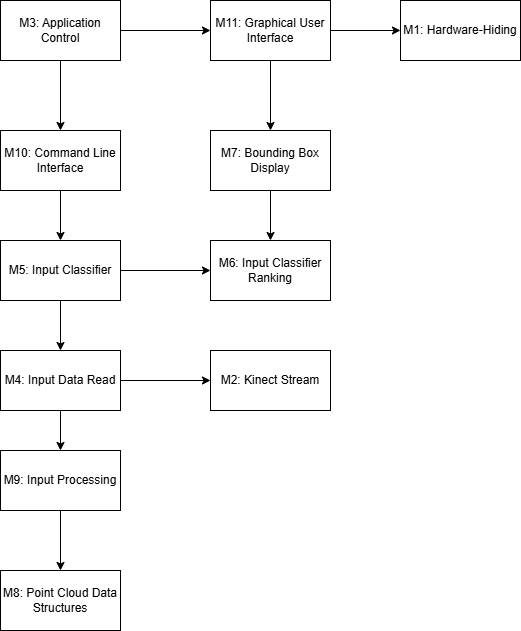
\includegraphics[width=0.7\textwidth]{ModuleHierarchy.png}
\caption{Use hierarchy among modules}
\label{FigUH}
\end{figure}

%\section*{References}

\section{User Interfaces}

\noindent \textbf{On First Run of Program:}\\
OS CLI window appears, prompting selection of Live (1) or Offline (2) modes. (Keyboard Interactive)\\

\noindent If Live (1) is selected:\\
Interactive viewer window (GUI) provided by the Point Cloud Library (PCL) will appear providing the resulting output from the feed.\\
\\

\noindent If Offline (2) is selected:\\
CLI window will prompt to paste in the full file path of the desired point cloud data file to be analyzed. 
Assuming a correct path and data provided, Interactive viewer window (GUI) provided by the Point Cloud Library (PCL) will appear providing the resulting output from the file.\\

\section{Design of Communication Protocols}

N/A

\section{Timeline}

Pending and future tasks can be viewed on the Kanban board hosted on \href{https://github.com/users/takhtart/projects/3}{GitHub}.

\bibliographystyle {plainnat}
\bibliography{../../../refs/References}

\newpage{}

\end{document}